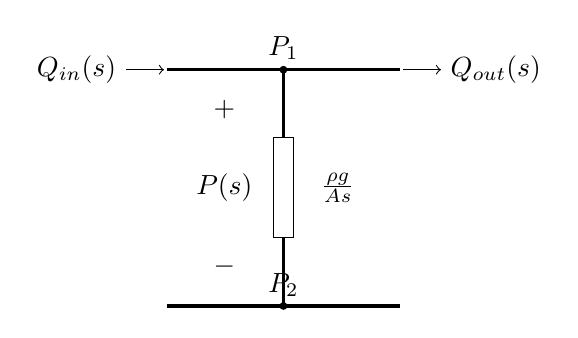
\begin{tikzpicture}
\draw (5.5,3.5) node[inner sep=0,outer sep=0] (a)  {};
\draw (5.5,0.5) node[inner sep=0,outer sep=0] (b) {};
\draw (8.5,3.5) node[inner sep=0,outer sep=0] (c) {};
\draw (8.5,0.5) node[inner sep=0,outer sep=0] (d) {};
%\draw (7,3.5) node[circle,draw,fill=black,inner sep=1pt] {} node[above] {$P_{1}$};
%\draw (7,0.5) node[circle,draw,fill=black,inner sep=1pt] {} node[below] {$P_{2}$};
\draw (6.25,3) node {$+$};
\draw (6.25,2) node {$P(s)$};
\draw (6.25,1) node {$-$};
\draw (7,2) node[rectangle,draw,minimum width=.1in,minimum height=.5in] (C) {};
\draw (C) node[right=10pt] {$\Huge\frac{\rho g}{As}$};
\draw (7,3.5) node[circle,fill,inner sep=1pt,] {} node[above] {$P_{1}$};
\draw[very thick] (a) -| (C.90);
\draw[very thick] (C.90) |- (c);
\draw[very thick] (b) -| (C.-90);
\draw[very thick] (C.-90) |- (d);
\draw (7,0.5) node[circle,fill,inner sep=1pt,] {} node[above] {$P_{2}$};
\draw[<-] (a) -- ++(-.5,0) node[left] {$Q_{in}(s)$};
\draw[->] (c) -- ++(.5,0) node[right] {$Q_{out}(s)$};

\end{tikzpicture}
